\section{Iron}

I generated another softer ECP for Fe in the same scheme as ccECPs, labeled as ccECP-soft. The KE cutoff is about 700 Ry. Below is the atomic gaps and molecular transferability test. Original published ccECP is included there as comparison too.

The Fe ccECP-soft parameter is give below and can also be downloaded under ./ccECP-soft-param/ directory:\\
16 3  \\
2 2 4 \\
2 8.9890516 13.9428916  \\  
2 14.963588  189.50111  \\
2 9.9838449 25.8036121  \\
2 14.979791  95.801262  \\
1 12.000794  16.0  \\
3 9.9968683 192.012710  \\
2 9.4029511 -110.30045  \\
2 5.9990706 2.59183990  \\

\begin{figure*}[!htbp]
\centering
\begin{subfigure}{0.5\textwidth}
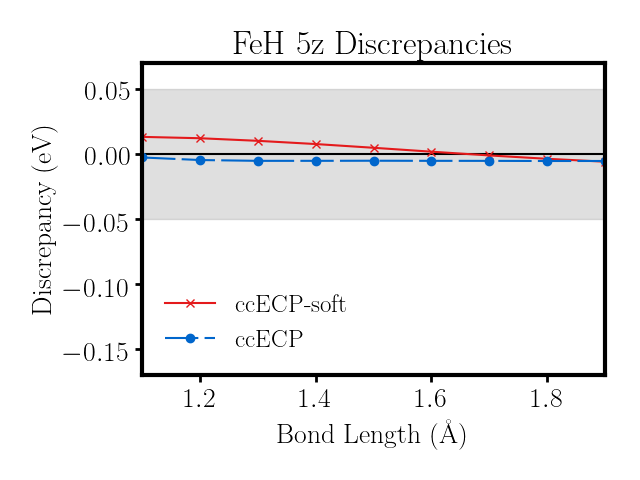
\includegraphics[width=\textwidth]{figures/FeH_5z.png}
\caption{FeH 5Z binding curve discrepancies}
\label{fig:FeO_5z}
\end{subfigure}%
\begin{subfigure}{0.5\textwidth}
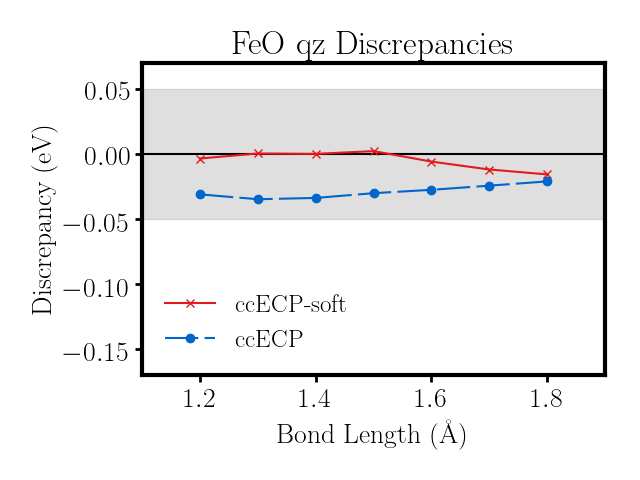
\includegraphics[width=\textwidth]{figures/FeO_qz.png}
\caption{FeO QZ binding curve discrepancies}
\label{fig:FeO_qz}
\end{subfigure}
\caption{Binding energy discrepancies for (a) FeH 5Z and (b) FeO QZ molecules with regard to CCSD(T). The shaded region indicates the band of chemical accuracy. The dashed vertical line represents the equilibrium geometry.}
\label{fig:Fe_mols}
\end{figure*}




\begin{table*}[!htbp]
\setlength{\tabcolsep}{3pt} %% default is 6pt
\centering
\caption{Fe gaps and relative errors for various ECPs.  All values in eV}
\resizebox{0.5\textwidth}{!}{%
\begin{tabular}{ll|cccccccccr}
\hline\hline
States and Symmetry &   &   AE &        ccECP   &   ccECP-soft  \\
\hline
{[Ar] $3d^74s^2$ } EA    & $^4F$ & -0.0579872 & -0.005436 &     -0.003053 \\
{[Ar] $3d^74s^1$ }       & $^5F$ &    0.88855 & -0.014150 &     -0.021149 \\
{[Ar] $3d^8$ }           & $^3F$ &    4.15711 & -0.017024 &     -0.019415 \\
{[Ar] $3d^64s^1$ }       & $^6D$ &    7.88583 & -0.016111 &     -0.034720 \\
{[Ar] $3d^7$ }           & $^4F$ &    8.16252 & -0.002125 &     -0.044298 \\
{[Ar] $3d^6$ }   2nd Ion & $^5D$ &    24.0909 &  0.013863 &     -0.041475 \\
{[Ar] $3d^5$ }   3rd Ion & $^5S$ &    54.6615 &  0.021912 &      0.005008 \\
\hline
MAD & &                                     &  0.012946 &      0.024160 \\
\hline
\hline
\end{tabular}
}
\end{table*}